\documentclass[10pt]{article}
\usepackage{amsmath}
\usepackage{cancel}
\usepackage{geometry}
\usepackage{graphicx}
\graphicspath{ {./images/} }
\geometry{legalpaper, margin=1.25in}
\usepackage[parfill]{parskip}

\setlength{\parindent}{0pt}



\title{1D FVM Moving Shock}
\author{Tristan Ball}


\begin{document}
	
	FVM moving shock in 1D with upwind flux. 
	
	\begin{figure}[h]
		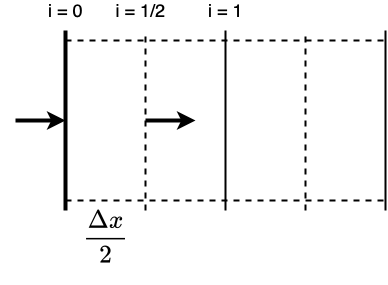
\includegraphics[width=8cm]{1D_FVM.png}
		\centering
	\end{figure}
	
	\begin{equation}
		\frac{\partial \mathbf{w} J}{\partial \tau} = F_{in} - F_{out}
	\end{equation}
	
%	\begin{equation}
%		\frac{\partial \mathbf{w} J}{\partial \tau} = 
%		\left[
%		\begin{tabular}{c}
%			$\rho u$ \\ $\rho u^2+P$ \\ $\rho u H$ 
%		\end{tabular}
%		\right]
%		- x_\tau
%		\left[
%		\begin{tabular}{c}
%			$\rho$\ \\ $\rho u$ \\ $\rho E$ 
%		\end{tabular}
%		\right]
%		- 
%	\end{equation}
	\begin{equation}
		\frac{\partial \mathbf{w} J}{\partial \tau} = (\mathbf{F}(\mathbf{\bar{w}}_u) - x_\tau \mathbf{\bar{w}}_u) - \left(\frac{\mathbf{F}(\mathbf{w}_1) + \mathbf{F}(\mathbf{w}_0)}{2} - |A|\frac{\mathbf{w}_1- \mathbf{w}_0}{2} \right)
	\end{equation}
	
	Define J as
	\begin{equation}
		J = \frac{\Delta x}{2} - x'
	\end{equation}
	
	Perturb w
	\begin{equation}
		\mathbf{w} = \bar{\mathbf{w}} + \mathbf{w}'
	\end{equation}
	
	Substitute and cancel $\bar{\mathbf{F}}$
	\begin{equation}
		\frac{\partial}{\partial \tau} \left( \left(\bar{\mathbf{w}} + \mathbf{w}'\right)\left(\frac{\Delta x}{2} - x'\right) \right) = 
	\end{equation}
	
	
\end{document}